%%%%%%%%%%%%%%%%%%%%%%%%%%%%%%%%%%%%%%%%%%%%%%%%%%%%%%%%%%%%%%%%%%%%%%%%%
% Template for a revtex article
%%%%%%%%%%%%%%%%%%%%%%%%%%%%%%%%%%%%%%%%%%%%%%%%%%%%%%%%%%%%%%%%%%%%%%%%%
\documentclass[rmp]{revtex4}
%%%%%%%%%%%%%%%%%%%%%%%%%%%%%%%%%%%%%%%%%%%%%%%%%%%%%%%%%%%%%%%%%%%%%%%%%
\usepackage[english]{babel}
\usepackage[utf8x]{inputenc}
\usepackage{amsmath,amsfonts,amssymb,eucal,eurosym,textcomp}
\usepackage{color}
\usepackage{graphicx}
\usepackage[caption=false]{subfig}
\usepackage{natbib}
\usepackage{pslatex}
\usepackage[colorlinks,linkcolor=red,citecolor=red]{hyperref}
%%%%%%%%%%%%%%%%%%%%%%%%%%%%%%%%%%%%%%%%%%%%%%%%%%%%%%%%%%%%%%%%%%%%%%%%%
\graphicspath{{./figures/}}
%%%%%%%%%%%%%%%%%%%%%%%%%%%%%%%%%%%%%%%%%%%%%%%%%%%%%%%%%%%%%%%%%%%%%%%%%
\newcommand{\comment}[1]{{\color{red}#1}}
%%%%%%%%%%%%%%%%%%%%%%%%%%%%%%%%%%%%%%%%%%%%%%%%%%%%%%%%%%%%%%%%%%%%%%%%%
\renewcommand{\thesubfigure}{\Alph{subfigure}}
\newcommand{\Author}{Fabio~Zanini* and Richard~A.~Neher*}
\newcommand{\Title}{Deleterious synonymous mutations hitchhike to high frequency in HIV \env~evolution}
\newcommand{\Affiliation}{Max Planck Institute for Developmental Biology, 72076 T\"ubingen, Germany}
%%%%%%%%%%%%%%%%%%%%%%%%%%%%%%%%%%%%%%%%%%%%%%%%%%%%%%%%%%%%%%%%%%%%%%%%%
\begin{document}
%%%%%%%%%%%%%%%%%%%%%%%%%%%%%%%%%%%%%%%%%%%%%%%%%%%%%%%%%%%%%%%%%%%%%%%%%
\title{\Title}
\author{\Author}
\affiliation{\textsf{*}\Affiliation}
\date{\today}
\maketitle
%%%%%%%%%%%%%%%%%%%%%%%%%%%%%%%%%%%%%%%%%%%%%%%%%%%%%%%%%%%%%%%%%%%%%%%%%
\tableofcontents

%%%%%%%%%%%%%%%%%%%%%%%%%%%%%%%%%%%%%%%%%%%%%%%%%%%%%%%%%%%%%%%%%%%%%%%%%
\section{Selection of the patient data}
%%%%%%%%%%%%%%%%%%%%%%%%%%%%%%%%%%%%%%%%%%%%%%%%%%%%%%%%%%%%%%%%%%%%%%%%%
\begin{figure}[ht]
\begin{center}
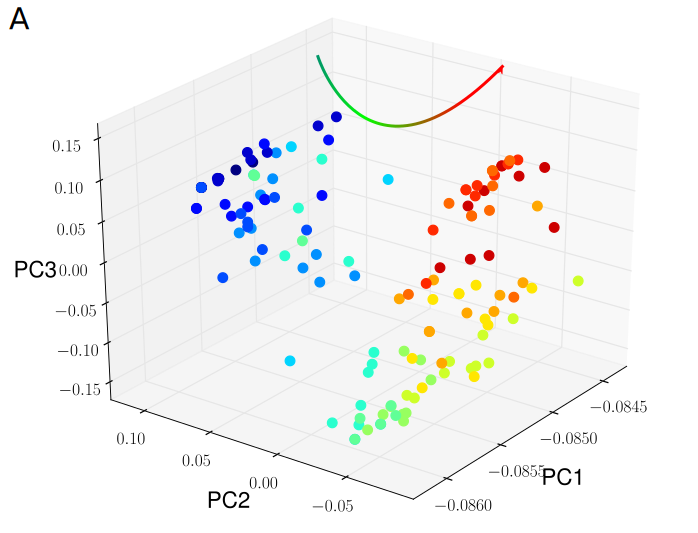
\includegraphics[width=0.35\linewidth]{Shankarappa_PCA_p1}
\includegraphics[width=0.35\linewidth]{Shankarappa_allele_freqs_trajectories_nonsyn_p1}
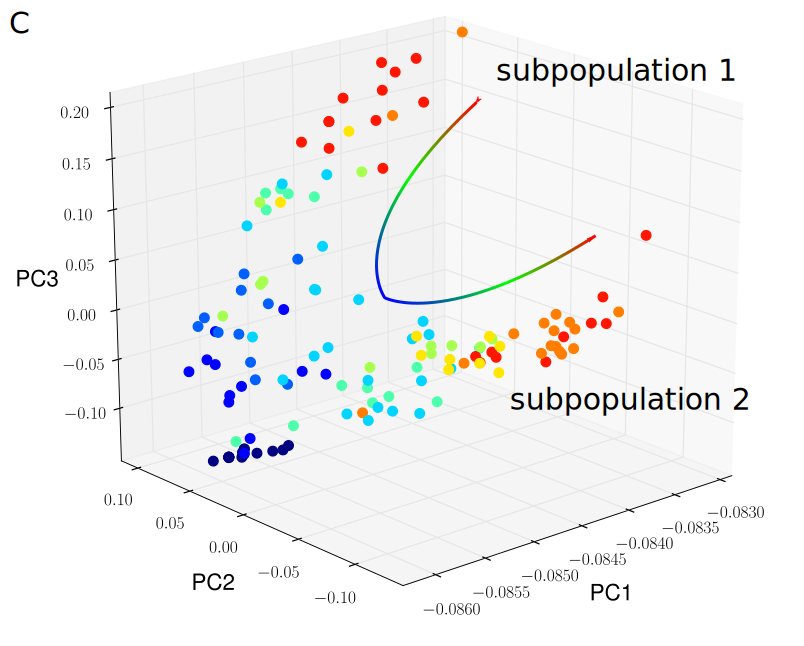
\includegraphics[width=0.35\linewidth]{Shankarappa_PCA_p7}
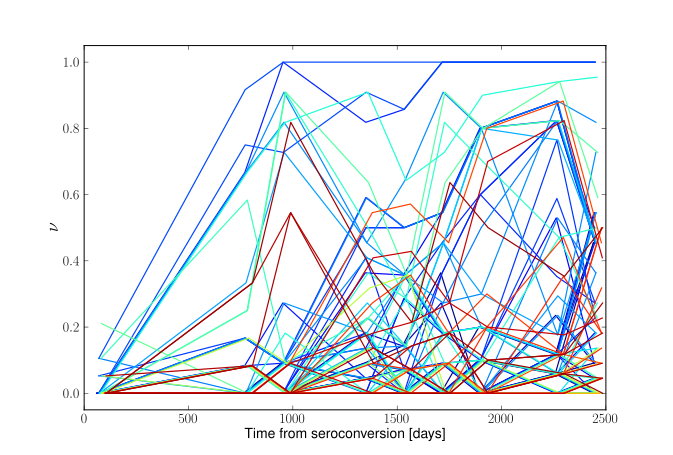
\includegraphics[width=0.35\linewidth]{Shankarappa_allele_freqs_trajectories_nonsyn_p7}
\caption{Panel A) PCA of all sequences from patient p1 (colors indicate time from seroconversion,
from blue to red). Panel B) Allele frequency trajectories for nonsynonymous
changes in the same patient. Panels C and D) show analogous plots for data from
patient p7. Samples after day 1000 split into two clusters in the PCA and no
mutations that arise after day 1000 fix, presumably because they are restricted
to one subpopulation. All patients like p7 (p4, p7, p8, p9 from ref.~\citealp{shankarappa_consistent_1999} and
ACH19542 and ACH19768 from ref.~\citealp{bunnik_autologous_2008}) were excluded
from our analysis.}
\label{fig:aftp}
\end{center}
\end{figure}

%%%%%%%%%%%%%%%%%%%%%%%%%%%%%%%%%%%%%%%%%%%%%%%%%%%%%%%%%%%%%%%%%%%%%%%%%
\section{Nonsynonymous changes outside of variable regions are deleterious}
%%%%%%%%%%%%%%%%%%%%%%%%%%%%%%%%%%%%%%%%%%%%%%%%%%%%%%%%%%%%%%%%%%%%%%%%%
\begin{figure}[h]
\begin{center}
\includegraphics[width=0.5\linewidth]{synmut_conservation_4fold_synnonsyn}
\caption{Cumulative distribution of synonymous and nonsynonymous diversity in
{\it gag} in the LANL reference panel(filtered
sequences only, version 2011)~\cite{LANL2012}. Sites such that the consensus codon
has three synonymous and six nonsynonymous single mutants were used, and the number of observed mutants
of a certain type over the number of possible mutants is plotted. Nonsynonymous
changes are observed less often, {\it ergo} are more conserved, than
synonymous changes. It can be therefore assumed, as mentioned in the main text,
that non-escape nonsynonymous changes involve a large fitness cost.}
\label{fig:synnonsyncons}
\end{center}
\end{figure}

%%%%%%%%%%%%%%%%%%%%%%%%%%%%%%%%%%%%%%%%%%%%%%%%%%%%%%%%%%%%%%%%%%%%%%%%%
\section{Synonymous diversity across the HIV genome}
%%%%%%%%%%%%%%%%%%%%%%%%%%%%%%%%%%%%%%%%%%%%%%%%%%%%%%%%%%%%%%%%%%%%%%%%%
\begin{figure}[h]
\begin{center}
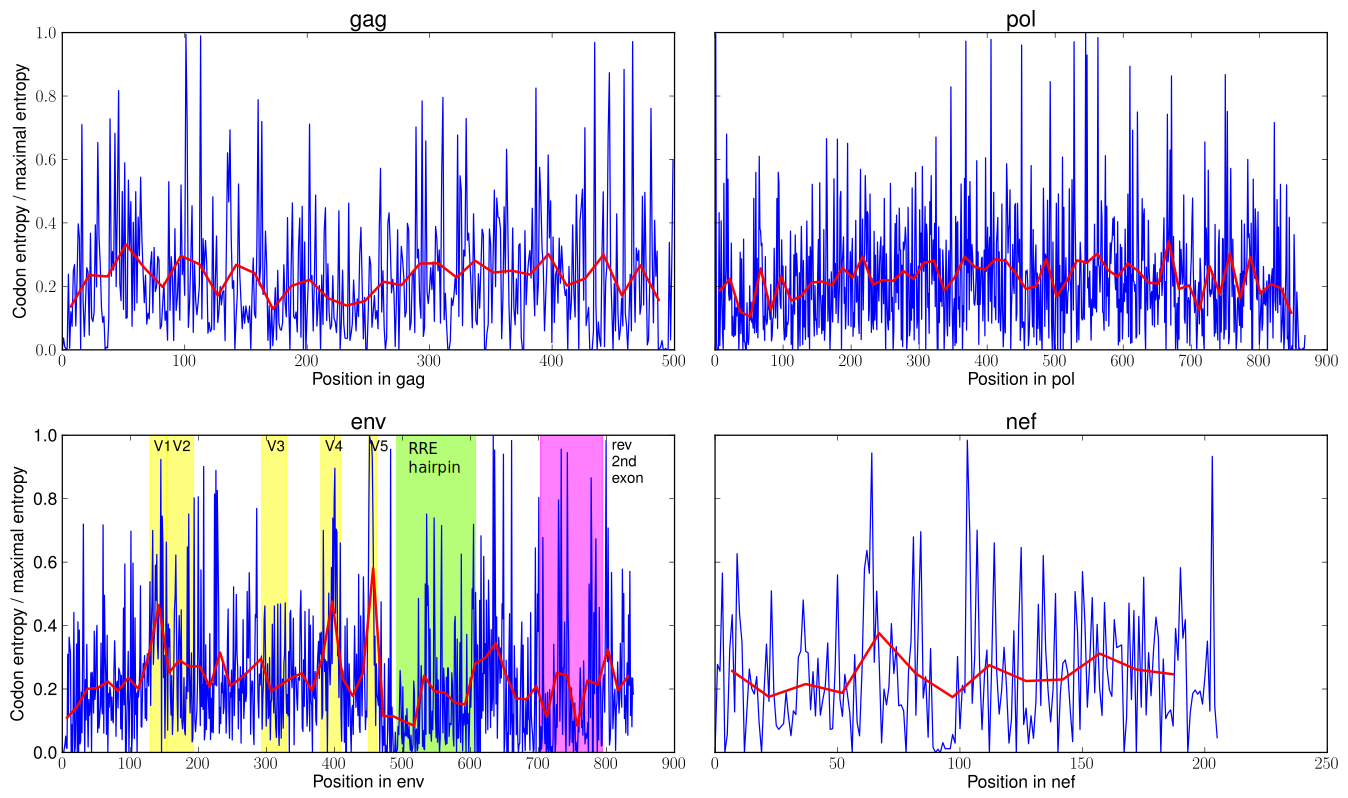
\includegraphics[width=\linewidth]{conservation_codons_genome}
\caption{Normalized codon entropy across the HIV genome is clustered around
variable regions in {\it env}. hence the synonymous mutational space is explored
deeper by HIV in that region, and even deleterious synonymous mutations can
reach high frequencies.
On the contrary, regions that are under purifying selection either
the the RNA level (the RRE hairpin) or at the protein level but in a different
reading frame (second {\it rev} exon, which includes the second {\it tat} exon),
show reduced entropy, i.e. more constrains.
All parts of {\it env} that are part of a different gene (signaling peptide,
second {\it rev} exon) have been excluded from our main analysis, to avoid
contamination about synonymity.
Data from a multiple sequence alignment of subtype-B HIV sequences from the LANL
website (filtered sequences only, version 2011)~\cite{LANL2012}.}
\label{fig:syndiv_genome}
\end{center}
\end{figure}

\clearpage

%%%%%%%%%%%%%%%%%%%%%%%%%%%%%%%%%%%%%%%%%%%%%%%%%%%%%%%%%%%%%%%%%%%%%%%%%
\section{Alternative models for suppression of nonsynonymous mutations}
%%%%%%%%%%%%%%%%%%%%%%%%%%%%%%%%%%%%%%%%%%%%%%%%%%%%%%%%%%%%%%%%%%%%%%%%%
\begin{figure}[h]
\begin{center}
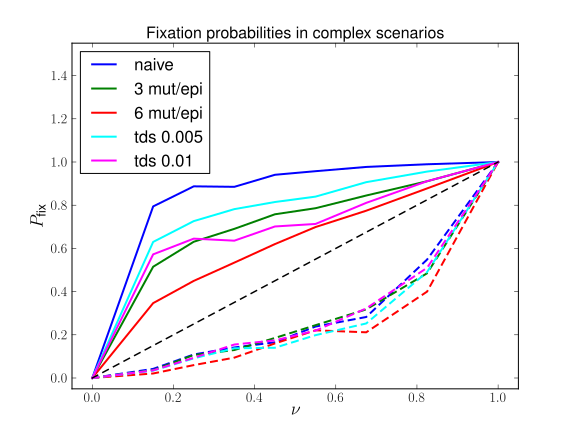
\includegraphics[width=0.5\linewidth]{simulations_graduallyepitopesandtimeselec}
\caption{Time-dependent selection (the escape mutant is recognized after some
months from its appearance) and competition between escape mutations in the same
epitope both reduce fixation of nonsynonymous mutations, without affecting the
synonymous curve much. In the
curves denoted with ``tds'' (time-dependent selection), the fitness advantage of
an escape mutaition can vanish at each time point with a probability density
\[ P_\text{recognized}(t) = c \cdot \nu(t), \]
where $c$ is a constant coefficient shown in the legend that encodes the overall
efficiency of the host immune system, and $\nu(t)$ is the frequency of the
escape allele at time $t$. The curves denoted with ``mut/epi'' describe the
competition scenario instead, with 3 or 6 escape mutations within the same
epitope of length 9 nucleotides.}
\label{fig:tds_wec}
\end{center}
\end{figure}
%%%%%%%%%%%%%%%%%%%%%%%%%%%%%%%%%%%%%%%%%%%%%%%%%%%%%%%%%%%%%%%%%%%%%%%%%
\bibliographystyle{natbib}
\bibliography{bib}
%%%%%%%%%%%%%%%%%%%%%%%%%%%%%%%%%%%%%%%%%%%%%%%%%%%%%%%%%%%%%%%%%%%%%%%%%
\end{document}
%%%%%%%%%%%%%%%%%%%%%%%%%%%%%%%%%%%%%%%%%%%%%%%%%%%%%%%%%%%%%%%%%%%%%%%%%

